\chapter{User Study}
\label{ch:user-study}

\section{Participants}
\label{sec:participants}
In total, 25 volunteers participated in this study, where 13 of them were male and 12 female students.
The sample was drawn from university populations having an age range from 19 to 31
years with a mean age of M = 26.12 (SD = 3.1).
Participants were selected from various discipline areas (see Figure~\ref{fig:Dfields}).
We consider academic disciplines as three categories (Social, Natural, and Formal Science)
where almost 30\% of participants are from the social sciences and 70\% from formal sciences.
Moreover, the participants had different education levels: the majority of
them were studying Masters’s degrees, and only 32 percent were Bachelors’s
and Ph.D.\ level students (see Figure~\ref{fig:DstudyLevels}).

\begin{figure}[H]
  \centering
    \includegraphics[scale=0.45]{RplotDemographicsFields.pdf}
      \caption{Participants' majors obtained from Demographics questionnaires}
      \label{fig:Dfields}
\end{figure}

\begin{figure}[H]
  \centering
    \includegraphics[scale=0.45]{RplotDemographicsStudyLevel.pdf}
      \caption{Participants' education level obtained from Demographics questionnaires}
      \label{fig:DstudyLevels}
\end{figure}

In the demographics form, participants also informed how frequently they used such devices as phones,
smart lamps, tablets, and speakers (see Figure~\ref{fig:DdeviceUse} and Figure~\ref{fig:DdeviceUseInHours}).

\begin{figure}[H]
  \centering
    \includegraphics[scale=0.45]{RplotDemographicsDeviceUse.pdf}
      \caption{Participants' use of devices obtained from Demographics questionnaires.}
      \label{fig:DdeviceUse}
\end{figure}

Overall, the experience level with the above-mentioned devices is listed in
descending order: phone, speakers, tablet, and smart lamps.
Figure~\ref{fig:DdeviceUseInHours} shows how many hours participants spend on these devices per day.
The demographics questionnaire showed that the most popular device among our participants
was a phone with approximately 1/3 of participants who spent more than 6 hours on them.
In all time ranges, the speakers were the second most used devices in
comparison to the number of participants using a tablet and smart lamps.

\begin{figure}[H]
  \centering
    \includegraphics[scale=0.45]{RplotDemographicsDeviceUseInHours.pdf}
      \caption{Participants' device use in hours obtained from Demographics questionnaires.}
      \label{fig:DdeviceUseInHours}
\end{figure}

In addition, Table~\ref{table:MusicFamiliarity} describes the participants’ preference for the music genres.
The more fluent the participant would be with the music, the more rapid
becomes the assessment of genre-specific features ~\cite{gjerdingen2008scanning}.
Moreover, if the majority of participants prefer to listen to or like a certain
genre of music, it may result in biased opinions.
The mascot that triggers genre that they prefer may give participants a more positive impression about their personality.
Thus, the main reason for gathering data regarding participants' music preferences
was to see whether the liking factor affects the study or not.

According to the One-Sample t-test with p>.05, there was no significant
effect of the participants’ music preference on the music genres that we chose for our study.
Thus, we have insufficient evidence to conclude that one music genre is more preferable than the other.
Meaning that, among the genres of music that we have chosen for our experiments,
there were no distinguishably favorite genres and the participants
had different music tastes (see Table~\ref{table:MusicFamiliarity}).

\begin{table}
\centering
\begin{tabular}{ | c | c| c | c | c | c | c |  }
\hline
\multirow{2}{*}{} &
  \multicolumn{1}{| c}{ t-value} &\multicolumn{1}{| c}{df}  & \multicolumn{1}{| c}{mean}
& \multicolumn{1}{| c}{p-value} & \multicolumn{2}{| c |}{95 percent confidence interval} \\
\hline
            &         &	      &	      &         &lower        &upper \\
\hline 
Country     &1        & 24    &.04    &.32      &-.04     &.12 \\
\hline 
Pop         &3.7      &24     &.36	  &.001     &.15	  &.57 \\
\hline 
Hip-hop	    &1.8	  &24	  &.12	  &.08	    &-.02	  &.26 \\
\hline 
Rap	        &1        &24     &.04	  &.33      &-.04     &.12\\
\hline 
Jazz        &2.4      &24     &.2     &.022     &.03      &.37\\
\hline 
Classic     &3.1      &24     &.28    &.005     &.09	  &.47\\
\hline 
Rock\&Roll  & 1	      &24	  &.04	  &.32	    &-.04     &.12\\
\hline 

\end{tabular}
\caption[]{T-test for participants' familiarity with music genres used in our study\footnotemark.}
\label{table:MusicFamiliarity}
\end{table}

\section{Procedure and Tasks}
\label{sec:procedure-and-tasks}
When the experiment started, the following aspects were described to the participants:
\begin{itemize}
  \item The implemented system introducing the devices used in this study.
  \item The key idea of a study.
  \item The purpose of the experiment.
  \item The goal of the participants during the experiment.
  \item The number of phases and the overall duration of the experiment.
\end{itemize}

\footnotetext{Note: Decimal points are omitted.}

In general, we have 4 phases for each interaction type such as mascot-mascot,
mascot-lamps, mascot-tablet, and mascot-speakers.
The order of all phases was counterbalanced by using Latin Square.
Each phase consists of 5 videos with a duration of 20 seconds, except for mascot-speakers
interactions where we have 9 videos with duration 40 seconds long.
Moreover, for each participant, there was a different order of displaying the videos
which are also randomized inside each phase based on the Latin Square.
All phases and all videos within those phases were counterbalanced across all participants.
Moreover, each participant was tested alone to ensure that the opinions of other participants do not affect their own.

Before each phase, we describe the participant what kind of interaction they should
expect from video and remind them of their goals during that experiment.
The goal is that, after watching short videos, participants will need to evaluate the personality
of a mascot according to the interaction that they have seen in the videos.
When accomplishing watching the video, the participants were given a questionnaire
(see appendix B) with 30 Likert scale questions and were asked to rank the personality trait
on a scale of 'Strongly Inaccurate' to 'Strongly Accurate'.
When this is done, the experiment continues to the next video.
After accomplishing watching all the videos in one phase, we move forward to the next phase.

In addition, the only phase where the participants are given an extra smartphone
is the mascot-mascot interaction phase, where two mascots start to vibrate
with a different duration based on the personality of approaching mascot.
Since it is difficult to see or hear the vibration from the videos, the phone runs an
application to simulate the different levels of a vibration that we showed participants in the video.
After watching the video, the participants were again given a questionnaire to assess
the personality of a mascot based on the video that they have seen and the vibration that they have felt.

Figure~\ref{fig:ExperimentPic} shows the screenshots of the videos that
participants watched during each phase of the experiment.
The pictures at the top represent the mascot-mascot and the mascot-lamp interaction
and the pictures at the bottom display the mascot-tablet and mascot-speakers interactions.

\begin{figure}[hbt!]
  \centering
  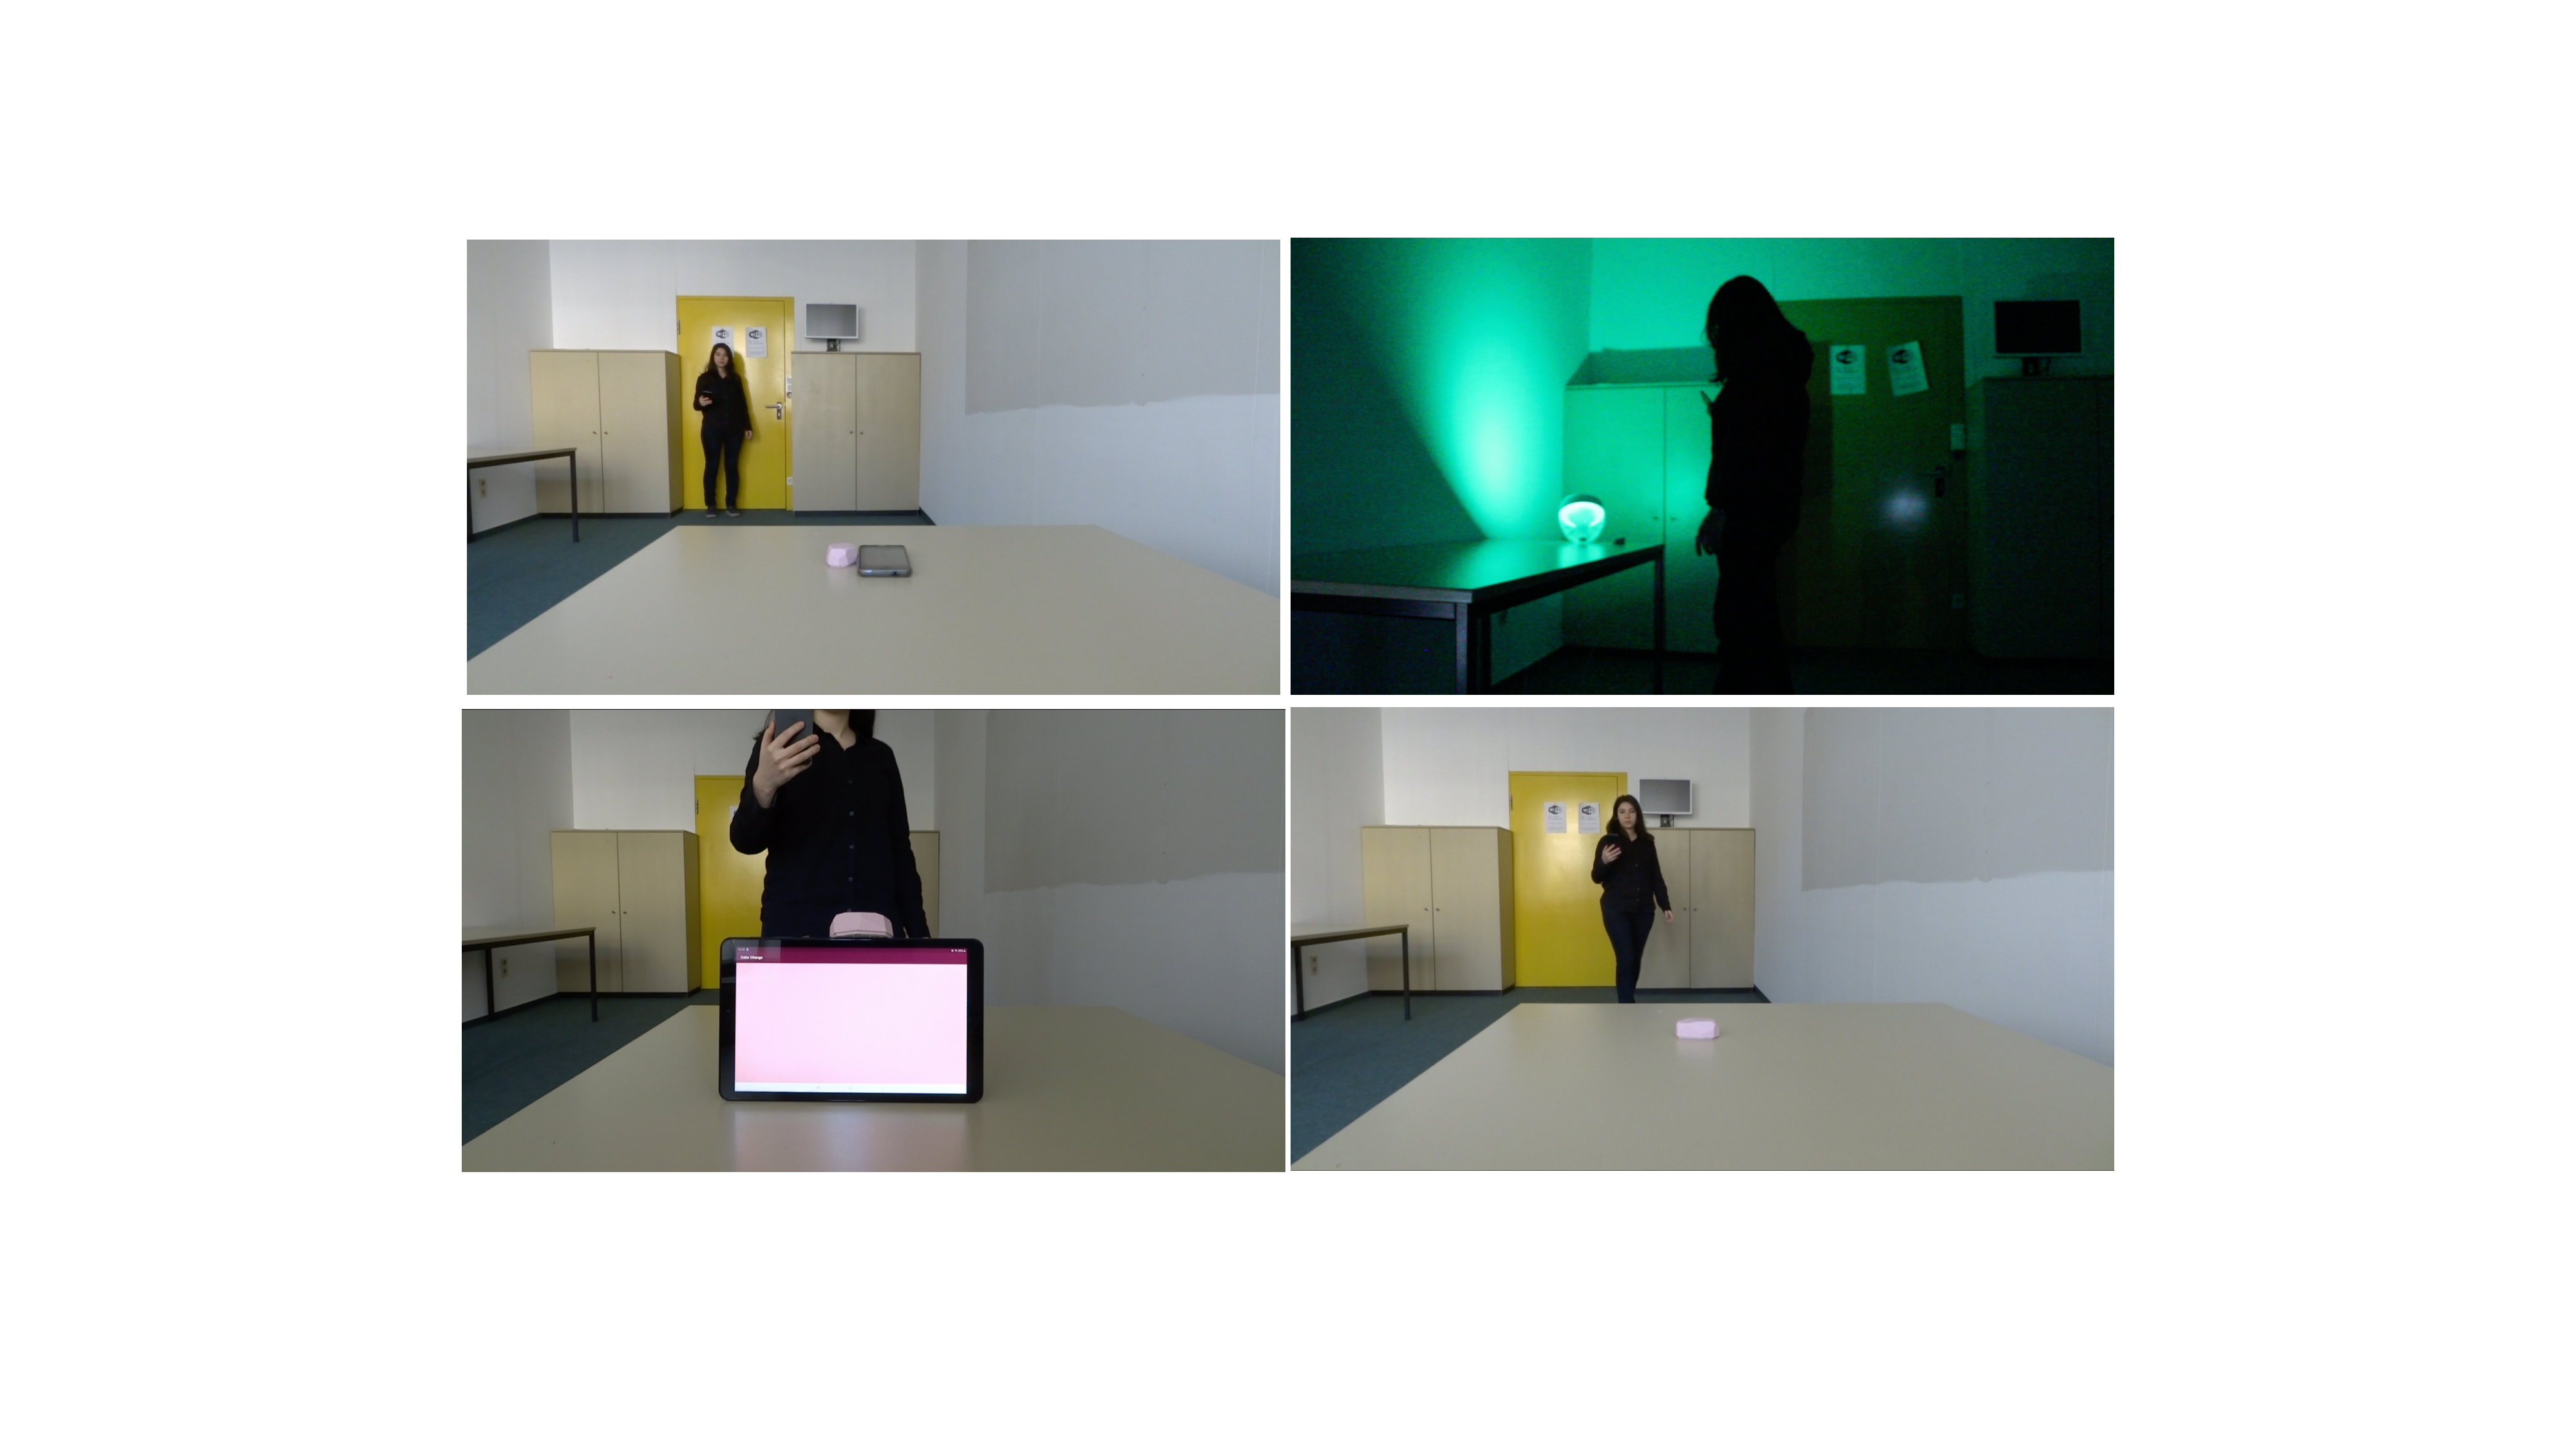
\includegraphics[scale=0.14]{ExperimentPic.jpg}
  \caption[]{The snapshots of videos from each case-study presented to the participants\footnotemark.}
  \label{fig:ExperimentPic}
\end{figure}
\footnotetext{During the experiments, the faces in the videos were not hidden,
for this document we hide faces with a nice smiley icon.}

After finishing the experiment, the participants were given a demographic questionnaire
with general information about themselves and their preferences.
The reason for giving this questionnaire at the end of the experiment was
not to affect the opinion of the participants.
Giving personal questions up-front, respondents could feel concerned that their personal
information is going to be linked to the experiment, and therefore, knowing which
characteristics will be taken into the account by the researchers, they may try
to fit their responses to the demographic questions that they filled.

The experiment, overall, lasts from one hour to an hour and a half, depending
on the speed of participants to fill the questionnaires.

\section{Design of experiments}
\label{sec:design-of-experiments}

It should be noted that as a design of the experiment we did not include a
real-life interaction with the devices, but instead, we showed participants videos
containing the interaction between social devices.
The main reason for that was the distraction of participants on various factors.

From an implementation perspective, the application using BLE - low-energy Bluetooth
technology measures the distance between objects with high accuracy and precision.
It can measure the distance from the smartphone to the beacon tag with
a margin error of 0.5 meters which is a
very good result\footnote{\url{https://altbeacon.github.io/android-beacon-library/distance-calculations.html}}.
However, the step of a person covers several centimeters at once, and the
application calculates each of these centimeters at a time.
Since asking participants to move slower or with small steps might distract
them by focusing on their behavior rather than on the assessment of the
mascot's personality, we decided to use videos in our experiments.
Moreover, these limitations are present in other applications that use BLE for calculating the distance.

Another factor that affects the study might be the vibration level during the mascot-mascot interaction.
In this study, we focus only on the duration of the vibration varying from 100 to 500 milliseconds per time.
Whenever a user interacts with the other mascot, the smartphone starts to vibrate with a particular duration.
Restricting participants to interact with the mascots with a specific number of times, might also shift
their focus, i.e\ instead of paying attention to the mascot's behavior, they will try to control their behavior.
Thus, to eliminate possible distracting factors, we decided to film all interactions between a
user and social devices, and show these videos to the participants.

Another design decision was instead of showing one video with all interaction types,
we split it into five short videos for mascot-lamp, mascot-table, mascot-mascot,
and into nine short videos for mascot-speakers interaction.
Despite the fact that the system supports multidimensional device interactions
i.e\ multiple mascots can interact with a lamp, a tablet, speakers, and other mascots at the same time,
we decided to split interaction types into four phases.
The main goal was to help participants to focus on one interaction and make
it easier for them to evaluate the personality of mascot based on a specific interaction type.

\section{Apparatus and Materials}
\label{sec:apparatus-and-materials}
The experiment’s setup consisted of the following devices:
\begin{itemize}
  \item MacBook Pro running Mac OS Catalina (Version 10.15.2).
  \item 55-inch monitor for displaying all videos.
  \item Tablet to fill the questionnaire in the google forms.
  \item Nexus One smartphone for simulating the vibration during mascot-mascot interaction.
\end{itemize}

As a survey tool for collecting data from participants, we used Google Form which consisted
of the thirty Likert scale type questions scaling from 'Strongly Inaccurate' to 'Strongly Accurate' scales.
Subsequently, in order to use obtained data in our statistical analysis, the questions
from our survey tool were transformed in a more permanent form (i.e four CSV files were generated, one for each phase,
and two CSV files for demographic questionnaire).

\section{Design of a study}
\label{sec:design-of-a-study}

The study consists of four case-studies: mascot-lamp, mascot-table, mascot-mascot, and mascot-speakers
interactions which, therefore, designed as four phases during experiments.
The experiment was a within-subjects design where each participant tests all conditions within each phase.
For example, for the mascot-lamp phase, each participant watches all five videos and
evaluates the personality of a mascot for each lighting color separately.
The within-subjects in comparison to the between-subjects design can help us to
reduce errors associated with individual differences.
Individual participants have different backgrounds, contexts, levels of concentration, and so on.
The same participant interacting with all 4 phases will affect the result in the same way
and can lower the probability that individual differences will skew the results.
Moreover, the within-subject design requires fewer participants, which may lead
us to the streamlined process of an experiment.

In this study, the independent variables (IVs) are factors that are triggered due to the behavior of a mascot.
For each case-study, we have a different number of IVs aka factors which are the followings:
\begin{itemize}
  \item For mascot-lamp case-study, there are five variables: turquoise, blood-red,
  yellow, orange, and pink lighting colors.
  \item For mascot-mascot case-study, five vibration levels: 100, 200, 300, 400, and 500 milliseconds per time.
  \item For mascot-speakers case-study, there are nine songs categorized into three variables:
        Sophisticated, Contemporary, and Unpretentious music categories.
   \item For mascot-tablet case-study, there are five variables: yellow, orange, turquoise,
        blood-red and pink background screen colors.
\end{itemize}

We do not compare case-studies with each other, where one interaction type
has a more effect on the measurements of the personality trait of mascots than the other type.
We consider one case as a separate study, where we only compare IVs.

Our dependent variable is the measurements of the personality traits based on the OCEAN model.
The main questions that we asked are the following:
\begin{itemize}
  \item Is the perception, namely, the measurements of the mascot’s personality affected by these factors?
  \item When they are affected, which personality traits does each factor convey?
\end{itemize}

\section{Measures}
\label{sec:measures}
As measurements of the experiments, we used questionnaires that were given after each video watch.
Overall, there were 24 questionnaires with five questionnaires in three phases and nine questionnaires
for the mascot-speakers interaction phase.
Each questionnaire consists of 30 questions portraying six facets of each personality based on the NEO-PIP survey.
The questionnaire items were answered using a Likert-scale
i.e.\ 'Very inaccurate', 'Inaccurate', 'Neutral', 'Accurate', 'Very accurate' rates.



